\documentclass{standalone}
\usepackage{tikz}
\usetikzlibrary{patterns, positioning}


\begin{document}
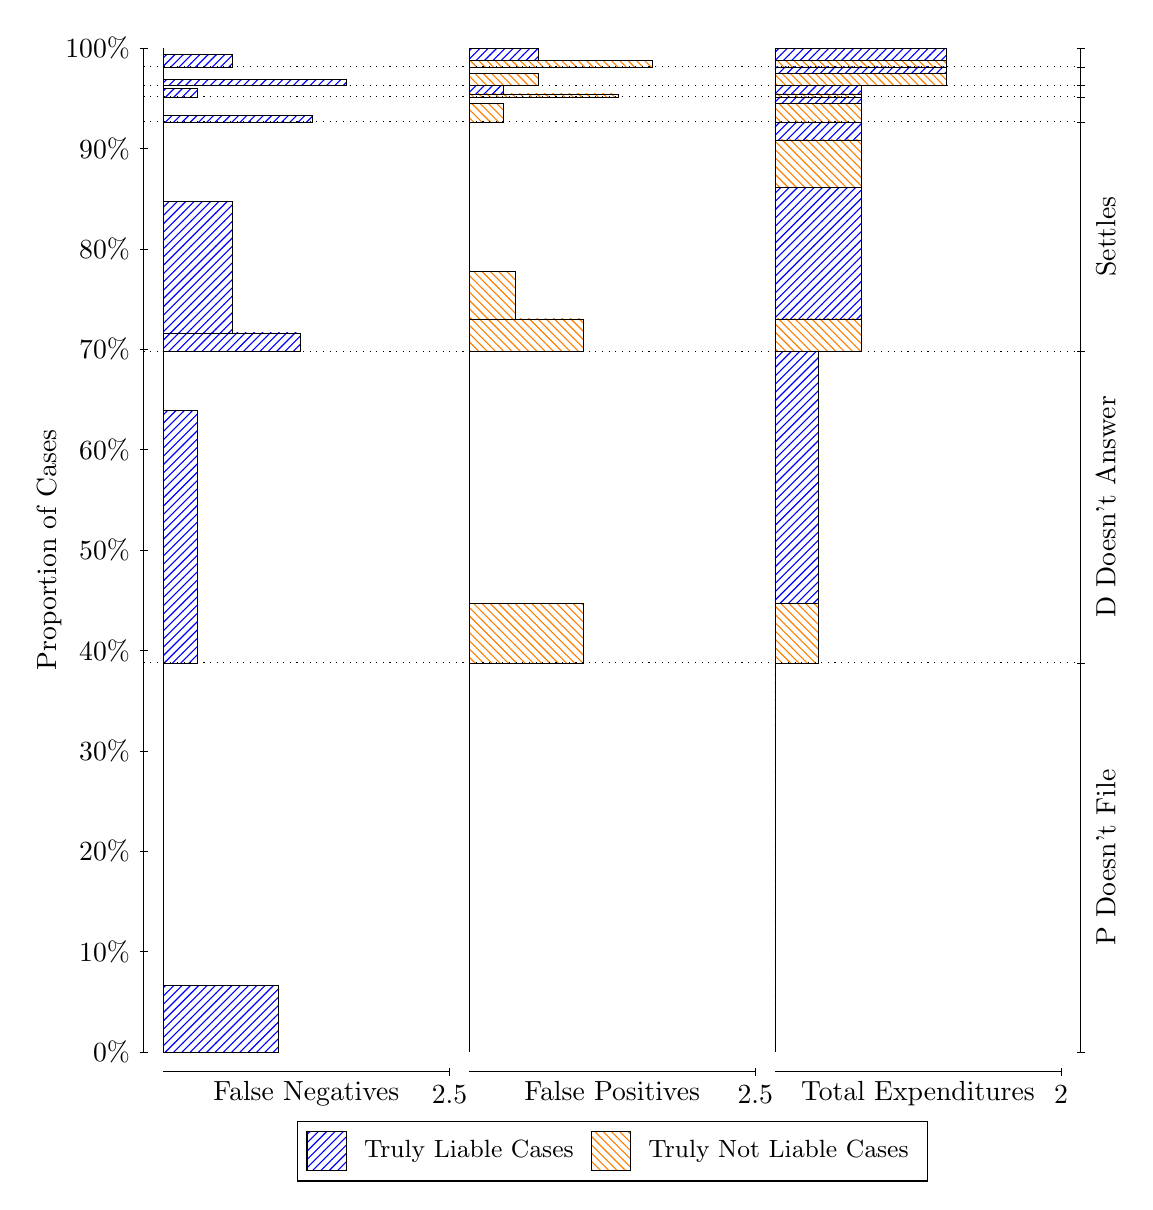
\begin{tikzpicture}
\draw[black, very thin] (1.5,1.75) -- (1.5,14.5);
\node[rotate=90, text=black, anchor=center] at (0.3, 8.125) {Proportion of Cases};
\draw[black, very thin] (1.45,1.75) -- (1.55,1.75);
\node[text=black, anchor=east] at (1.45, 1.75) {0\%};
\draw[black, very thin] (1.45,3.025) -- (1.55,3.025);
\node[text=black, anchor=east] at (1.45, 3.025) {10\%};
\draw[black, very thin] (1.45,4.3) -- (1.55,4.3);
\node[text=black, anchor=east] at (1.45, 4.3) {20\%};
\draw[black, very thin] (1.45,5.575) -- (1.55,5.575);
\node[text=black, anchor=east] at (1.45, 5.575) {30\%};
\draw[black, very thin] (1.45,6.85) -- (1.55,6.85);
\node[text=black, anchor=east] at (1.45, 6.85) {40\%};
\draw[black, very thin] (1.45,8.125) -- (1.55,8.125);
\node[text=black, anchor=east] at (1.45, 8.125) {50\%};
\draw[black, very thin] (1.45,9.4) -- (1.55,9.4);
\node[text=black, anchor=east] at (1.45, 9.4) {60\%};
\draw[black, very thin] (1.45,10.675) -- (1.55,10.675);
\node[text=black, anchor=east] at (1.45, 10.675) {70\%};
\draw[black, very thin] (1.45,11.95) -- (1.55,11.95);
\node[text=black, anchor=east] at (1.45, 11.95) {80\%};
\draw[black, very thin] (1.45,13.225) -- (1.55,13.225);
\node[text=black, anchor=east] at (1.45, 13.225) {90\%};
\draw[black, very thin] (1.45,14.5) -- (1.55,14.5);
\node[text=black, anchor=east] at (1.45, 14.5) {100\%};

\draw[black, very thin] (13.4,1.75) -- (13.4,14.5);
\draw[black, very thin] (13.35,1.75) -- (13.45,1.75);
\node[anchor=west] at (13.35, 1.75) {};
\draw[black, very thin] (13.35,6.6917) -- (13.45,6.6917);
\node[anchor=west] at (13.35, 6.6917) {};
\draw[black, very thin] (13.35,10.65) -- (13.45,10.65);
\node[anchor=west] at (13.35, 10.65) {};
\draw[black, very thin] (13.35,13.563) -- (13.45,13.563);
\node[anchor=west] at (13.35, 13.563) {};
\draw[black, very thin] (13.35,13.88) -- (13.45,13.88);
\node[anchor=west] at (13.35, 13.88) {};
\draw[black, very thin] (13.35,14.022) -- (13.45,14.022);
\node[anchor=west] at (13.35, 14.022) {};
\draw[black, very thin] (13.35,14.261) -- (13.45,14.261);
\node[anchor=west] at (13.35, 14.261) {};
\draw[black, very thin] (13.35,14.5) -- (13.45,14.5);
\node[anchor=west] at (13.35, 14.5) {};

\draw[black, very thin, pattern color=blue, pattern=north east lines] (1.75,1.75) rectangle (3.2033,2.5925);
\draw[black, very thin, pattern color=orange, pattern=north west lines] (1.75,2.5925) rectangle (1.75,6.6917);
\draw[black, very thin, pattern color=blue, pattern=north east lines] (1.75,6.6917) rectangle (2.186,9.8961);
\draw[black, very thin, pattern color=orange, pattern=north west lines] (1.75,9.8961) rectangle (1.75,10.65);
\draw[black, very thin, pattern color=blue, pattern=north east lines] (1.75,10.65) rectangle (3.494,10.881);
\draw[black, very thin, pattern color=blue, pattern=north east lines] (1.75,10.881) rectangle (2.622,12.552);
\draw[black, very thin, pattern color=orange, pattern=north west lines] (1.75,12.552) rectangle (1.75,13.563);
\draw[black, very thin, pattern color=blue, pattern=north east lines] (1.75,13.563) rectangle (3.6393,13.646);
\draw[black, very thin, pattern color=orange, pattern=north west lines] (1.75,13.646) rectangle (1.75,13.88);
\draw[black, very thin, pattern color=blue, pattern=north east lines] (1.75,13.88) rectangle (2.186,13.985);
\draw[black, very thin, pattern color=orange, pattern=north west lines] (1.75,13.985) rectangle (1.75,14.022);
\draw[black, very thin, pattern color=blue, pattern=north east lines] (1.75,14.022) rectangle (4.0753,14.106);
\draw[black, very thin, pattern color=orange, pattern=north west lines] (1.75,14.106) rectangle (1.75,14.261);
\draw[black, very thin, pattern color=blue, pattern=north east lines] (1.75,14.261) rectangle (2.622,14.416);
\draw[black, very thin, pattern color=orange, pattern=north west lines] (1.75,14.416) rectangle (1.75,14.5);
\draw[black, very thin, pattern color=orange, pattern=north west lines] (5.6333,1.75) rectangle (5.6333,5.8493);
\draw[black, very thin, pattern color=blue, pattern=north east lines] (5.6333,5.8493) rectangle (5.6333,6.6917);
\draw[black, very thin, pattern color=orange, pattern=north west lines] (5.6333,6.6917) rectangle (7.0867,7.4461);
\draw[black, very thin, pattern color=blue, pattern=north east lines] (5.6333,7.4461) rectangle (5.6333,10.65);
\draw[black, very thin, pattern color=orange, pattern=north west lines] (5.6333,10.65) rectangle (7.0867,11.059);
\draw[black, very thin, pattern color=orange, pattern=north west lines] (5.6333,11.059) rectangle (6.2147,11.662);
\draw[black, very thin, pattern color=blue, pattern=north east lines] (5.6333,11.662) rectangle (5.6333,13.563);
\draw[black, very thin, pattern color=orange, pattern=north west lines] (5.6333,13.563) rectangle (6.0693,13.798);
\draw[black, very thin, pattern color=blue, pattern=north east lines] (5.6333,13.798) rectangle (5.6333,13.88);
\draw[black, very thin, pattern color=orange, pattern=north west lines] (5.6333,13.88) rectangle (7.5227,13.917);
\draw[black, very thin, pattern color=blue, pattern=north east lines] (5.6333,13.917) rectangle (6.0693,14.022);
\draw[black, very thin, pattern color=orange, pattern=north west lines] (5.6333,14.022) rectangle (6.5053,14.176);
\draw[black, very thin, pattern color=blue, pattern=north east lines] (5.6333,14.176) rectangle (5.6333,14.261);
\draw[black, very thin, pattern color=orange, pattern=north west lines] (5.6333,14.261) rectangle (7.9587,14.345);
\draw[black, very thin, pattern color=blue, pattern=north east lines] (5.6333,14.345) rectangle (6.5053,14.5);
\draw[black, very thin, pattern color=orange, pattern=north west lines] (9.5167,1.75) rectangle (9.5167,5.8493);
\draw[black, very thin, pattern color=blue, pattern=north east lines] (9.5167,5.8493) rectangle (9.5167,6.6917);
\draw[black, very thin, pattern color=orange, pattern=north west lines] (9.5167,6.6917) rectangle (10.062,7.4461);
\draw[black, very thin, pattern color=blue, pattern=north east lines] (9.5167,7.4461) rectangle (10.062,10.65);
\draw[black, very thin, pattern color=orange, pattern=north west lines] (9.5167,10.65) rectangle (10.607,11.059);
\draw[black, very thin, pattern color=blue, pattern=north east lines] (9.5167,11.059) rectangle (10.607,12.731);
\draw[black, very thin, pattern color=orange, pattern=north west lines] (9.5167,12.731) rectangle (10.607,13.333);
\draw[black, very thin, pattern color=blue, pattern=north east lines] (9.5167,13.333) rectangle (10.607,13.563);
\draw[black, very thin, pattern color=orange, pattern=north west lines] (9.5167,13.563) rectangle (10.607,13.798);
\draw[black, very thin, pattern color=blue, pattern=north east lines] (9.5167,13.798) rectangle (10.607,13.88);
\draw[black, very thin, pattern color=orange, pattern=north west lines] (9.5167,13.88) rectangle (10.607,13.917);
\draw[black, very thin, pattern color=blue, pattern=north east lines] (9.5167,13.917) rectangle (10.607,14.022);
\draw[black, very thin, pattern color=orange, pattern=north west lines] (9.5167,14.022) rectangle (11.697,14.176);
\draw[black, very thin, pattern color=blue, pattern=north east lines] (9.5167,14.176) rectangle (11.697,14.261);
\draw[black, very thin, pattern color=orange, pattern=north west lines] (9.5167,14.261) rectangle (11.697,14.345);
\draw[black, very thin, pattern color=blue, pattern=north east lines] (9.5167,14.345) rectangle (11.697,14.5);
\draw[black, dotted] (1.5,6.6917) -- (13.4,6.6917);
\draw[black, dotted] (1.5,10.65) -- (13.4,10.65);
\draw[black, dotted] (1.5,13.563) -- (13.4,13.563);
\draw[black, dotted] (1.5,13.88) -- (13.4,13.88);
\draw[black, dotted] (1.5,14.022) -- (13.4,14.022);
\draw[black, dotted] (1.5,14.261) -- (13.4,14.261);
\draw[black, very thin] (1.75,1.5) -- (5.3833,1.5);
\node[text=black, anchor=north] at (3.5667, 1.5) {False Negatives};
\draw[black, very thin] (5.3833,1.45) -- (5.3833,1.55);
\node[text=black, anchor=north] at (5.3833, 1.45) {2.5};

\draw[black, very thin] (5.6333,1.5) -- (9.2667,1.5);
\node[text=black, anchor=north] at (7.45, 1.5) {False Positives};
\draw[black, very thin] (9.2667,1.45) -- (9.2667,1.55);
\node[text=black, anchor=north] at (9.2667, 1.45) {2.5};

\draw[black, very thin] (9.5167,1.5) -- (13.15,1.5);
\node[text=black, anchor=north] at (11.333, 1.5) {Total Expenditures};
\draw[black, very thin] (13.15,1.45) -- (13.15,1.55);
\node[text=black, anchor=north] at (13.15, 1.45) {2};

\node[text=black, centered, rotate=90] at (13.72, 4.2209) {P Doesn't File};
\node[text=black, centered, rotate=90] at (13.72, 8.6711) {D Doesn't Answer};
\node[text=black, centered, rotate=90] at (13.72, 12.107) {Settles};





\draw (7.449999999999999,1.5) node[draw=none] (baseCoordinate) {};
\begin{scope}[align=center]
        \matrix[scale=0.5, draw=black, below=0.5cm of baseCoordinate, nodes={draw}, column sep=0.1cm]{
            \node[rectangle, draw, minimum width=0.5cm, minimum height=0.5cm, pattern color=blue, pattern=north east lines] {}; &
            \node[draw=none, font=\small, text=black] (B) {Truly Liable Cases}; &
            \node[rectangle, draw, minimum width=0.5cm, minimum height=0.5cm, pattern color=orange, pattern=north west lines] {}; &
            \node[draw=none, font=\small, text=black] (B) {Truly Not Liable Cases}; \\
            };
\end{scope}

\end{tikzpicture}
\end{document}